%********************************************************************************
% Title: Performance Modeling of a Fog Computing System
%
% Series: Courseworks in Performance Modeling of Computer Systems and Networks
%
% Author: Giacomo Marciani <mgiacomo@amazon.com>
%
% Institution: Department of Civil Engineering and Computer Science Engineering,
% University of Rome Tor Vergata, Italy
%
% Style: ACM ART SIGCONFS (based on ACM Large v1.7)
%*******************************************************************************

\documentclass[sigconf]{acmart}

\usepackage[utf8]{inputenc}
\usepackage{booktabs}
\usepackage{algorithm2e}
\usepackage{listings}
\usepackage{color, soul}
\usepackage{graphicx}
\usepackage{lipsum}
\usepackage{epstopdf}
\usepackage{subfig}
\usepackage{bm}
\usepackage{url}
\usepackage{array}

%*******************************************************************************
% Packages setting
%*******************************************************************************
\graphicspath{{fig/}}

%*******************************************************************************
% Shared Affiliation format
%*******************************************************************************
\def\sharedaffiliation{%
\end{tabular}
\begin{tabular}{c}}

%*******************************************************************************
% Fonts
%*******************************************************************************
%\newfont{\eaddfntresz}{phvr8t at 11pt}

%*******************************************************************************
% Margins
%*******************************************************************************
%\clubpenalty=10000
%\widowpenalty=10000

%*******************************************************************************
% hyphenation
%*******************************************************************************
\hyphenation{sched-uler par-a-digm adopt-ed evolv-ing th}

%*******************************************************************************
% pseudocode customisation
%*******************************************************************************
%\makeatletter
%\def\BState{\State\hskip-\ALG@thistlm}
%\makeatother

%*******************************************************************************
% Details
%*******************************************************************************
\acmConference[PMCSN'20]{Performance Modeling of a Fog Computing System}{February 2021}{Rome, Italy}
\acmYear{2021}
\copyrightyear{2021}
\setcopyright{rightsretained}
\acmISBN{123-4567-24-567/08/06}
\acmDOI{10.475/123_4}
\acmPrice{15.00}

\begin{document}
%*******************************************************************************
% Title
%*******************************************************************************
\title{Performance Modeling of a Fog Computing System}

%*******************************************************************************
% Authors
%*******************************************************************************
\author{Giacomo Marciani}
\orcid{0000-0002-3675-8804}
\affiliation{%
  \institution{University of Rome Tor Vergata}
  \streetaddress{Via del Politecnico 1}
  \city{Rome}
  \state{Italy}
  \postcode{00133}
}
\email{mgiacomo@amazon.com}

\renewcommand{\shortauthors}{G. Marciani}

%*******************************************************************************
% Contents
%*******************************************************************************
\begin{abstract}
We prove the semi-decidability of the problem of saying whether or not a context-free grammar generates a regular language.
We introduce the notion of context-free grammar in Marciani Normal Form.
We prove that a context-free grammar in Marciani Normal Form always generates a regular language.
\end{abstract}

% http://dl.acm.org/ccs.cfm

\begin{CCSXML}
    <ccs2012>
    <concept>
        <concept_id>10003752.10003809.10003716</concept_id>
        <concept_desc>Theory of computation~Mathematical optimization</concept_desc>
        <concept_significance>500</concept_significance>
    </concept>
    <concept>
        <concept_id>10003752.10003809.10003716.10011136</concept_id>
        <concept_desc>Theory of computation~Discrete optimization</concept_desc>
        <concept_significance>500</concept_significance>
    </concept>
    <concept>
        <concept_id>10003752.10003809.10003716.10011138</concept_id>
        <concept_desc>Theory of computation~Continuous optimization</concept_desc>
        <concept_significance>500</concept_significance>
    </concept>
    <concept>
        <concept_id>10003752.10003809.10003716.10011141</concept_id>
        <concept_desc>Theory of computation~Mixed discrete-continuous optimization</concept_desc>
        <concept_significance>500</concept_significance>
    </concept>
    <concept>
        <concept_id>10003752.10003809.10003716.10011804</concept_id>
        <concept_desc>Theory of computation~Non-parametric optimization</concept_desc>
        <concept_significance>500</concept_significance>
    </concept>
    <concept>
        <concept_id>10010147.10010148.10010149.10010161</concept_id>
        <concept_desc>Computing methodologies~Optimization algorithms</concept_desc>
        <concept_significance>500</concept_significance>
    </concept>
    <concept>
        <concept_id>10010405.10010481</concept_id>
        <concept_desc>Applied computing~Operations research</concept_desc>
        <concept_significance>500</concept_significance>
    </concept>
    </ccs2012>
\end{CCSXML}

\ccsdesc[500]{Theory of computation~Mathematical optimization}
\ccsdesc[500]{Theory of computation~Discrete optimization}
\ccsdesc[500]{Theory of computation~Continuous optimization}
\ccsdesc[500]{Theory of computation~Mixed discrete-continuous optimization}
\ccsdesc[500]{Theory of computation~Non-parametric optimization}
\ccsdesc[500]{Computing methodologies~Optimization algorithms}
\ccsdesc[500]{Applied computing~Operations research}

\keywords{AMPL,CPLEX}

\maketitle
\section{Introduction}
\label{sec:introduction}

In \Cref{sec:definitions}, we give some preliminary definitions about language
equations and the regularity problem.
In particular, we introduce the class of bilateral-linear language equations,
the pseudo-regular partition of productions and the looking forward property.

In \Cref{sec:marciani-rule}, we state and prove Marciani's Rule, which exposes
a method to solve the bilateral-linear language equations.

In \Cref{sec:marciani-normal-form}, we define the Marciani Normal Form, and we
prove that a context-free grammar in such a form always generates a regular
language.

In \Cref{sec:semi-decidability}, we prove the semi-decidability and the
undecidability of the context-free regularity problem, by the application of the 
previous results.

In \Cref{sec:examples}, we give some applicative examples of the Marciani's Rule
and the Marciani Normal Form.

\section{Goals and Objectives}
\label{sec:performance-modeling-goals-and-objectives}
\textit{Performance modeling} is the art of studying the behavior of a system in terms of performance metrics in order to maximize the return on tech investments.
To this aim, the \textit{simulation} is the most effective and scalable way to gather system insights and prove performance conjectures without even requiring the existence of the real system.

In this paper, we consider the system architecture in Figure~\ref{fig:system-architecture} and use a simulator to study its behavior with the goal of minimizing the response time.

The system is made of two following layers and accepts classed end-user workloads:

\begin{itemize}
		\item \textbf{Cloudlet:} upfront layer made of one-hop finite resources, having the ability to off-load tasks to the Cloud server, accordingly to an \textit{off-loading policy} based on the occupancy state of the Cloudlet. In particular, the Cloudlet may \textit{forward} incoming tasks to Cloud or \textit{restart} preempted tasks in Cloud with some \textit{overhead}. 
		
		\item \textbf{Cloud:} backfront layer made of a remote Cloud server with virtually unlimited resources.
\end{itemize}

We assume the Cloudlet  providing tasks with higher service rates than the Cloud because, since the former is placed on the network edge, it has lower transmission time and it is less exposed to network latencies.

We propose to evaluate the system behavior with two alternative off-loading policies:

\begin{itemize}
	\item \textbf{Off-Loading Policy 1 (OP1):} the Cloudlet makes no distinction between tasks; it forwards incoming tasks to the Cloud when it has no available resources. Actually, OP1 represents the absence of an off-loading policy because in this case no off-loading is actually performed.
	
	\item \textbf{Off-Loading Policy 2 (OP2):} the Cloudlet gives higher priority to $1^{st}$ class tasks; it accepts only a dynamically thresholded occupancy of $2^{nd}$ class tasks, interrupts $2^{nd}$ class tasks to free up resources for $1^{st}$ class tasks and forwards incoming tasks to the Cloud when it has no available resources.
\end{itemize}

We propose to evaluate the convergence of the system to a steady state and the following performance metrics in the steady state with a $95\%$ level of confidence:

\begin{itemize}
	\item \textit{System/Cloudlet/Cloud response time} both global and per-class;
	
	\item \textit{System/Cloudlet/Cloud throughput} both global and per-class;
	
	\item \textit{System/Cloudlet/Cloud mean population} both global and per-class;
	
	\item \textit{Cloudlet interruption percentage} of the $2^{nd}$ class tasks;
	
	\item \textit{System response time of interrupted tasks}.
\end{itemize}

\begin{figure}
	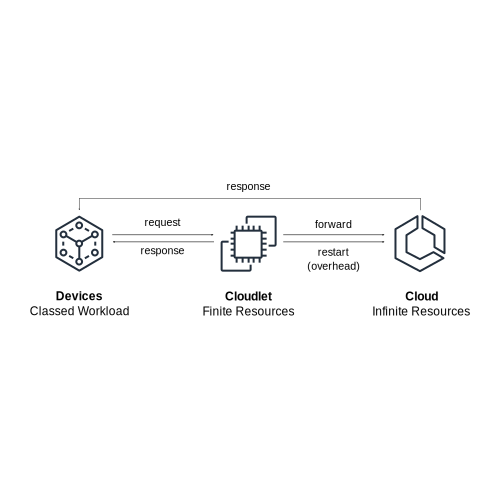
\includegraphics[width=\columnwidth]{fig/architecture}
	\caption{System architecture.}
	\label{fig:system-architecture}
\end{figure}

It is worth studying such a system because it represents the simplest form of a Fog Computing infrastructure, where the end-user workload is  served by Edge compute nodes,  possibly off-loading it to a Cloud provider. The goal of such a study is then to asses the impact of distinct off-loading policies given the trade-off between (i) Edge compute nodes, which are barely exposed to network latencies, but hardly scale and (ii) Cloud compute nodes,  which are virtually infinite, but more exposed to network latencies.
\section{Conceptual Model}
\label{sec:performance-modeling-conceptual-model}
A conceptual model defines the target system in terms of 
(i) the states it can assume over time, 
(ii) the events that let it change in time and
(iii) system assumptions.

We consider the conceptual model depicted in Figure~\ref{fig:conceptual-model-1} and \ref{fig:conceptual-model-2}, respectively for the system running the off-loading algorithm 1 and 2.
In both models, we introduced the \textit{Controller (CTRL)} component within the Cloudlet to represent the decision process of the off-loading policy.

\begin{figure}
	\includegraphics[width=\columnwidth]{fig/conceptual-model-1}
	\caption{Conceptual model of the system with with OP1.}
	\label{fig:conceptual-model-1}
\end{figure}

\begin{figure}
	\includegraphics[width=\columnwidth]{fig/conceptual-model-2}
	\caption{Conceptual model of the system with OP2.}
	\label{fig:conceptual-model-2}
\end{figure}

\paragraph{State space}
The state space $S$ of a system is a comprehensive characterization of the system at any given time.
The state space of the whole system is represented by the state space of its subsystems:

\begin{itemize}
	\item \textbf{Cloudlet}: $S_{clt} := \{(n_{clt,1},n_{clt,2})\in \mathcal{N}^{2}: n_{clt,1}+n_{clt,2}\leq N\}$, where $n_{clt,i}$ is the population of tasks belonging to the $i$-th class within the Cloudlet.
	
	\item \textbf{Cloud}: $S_{cld} := \{(n_{cld,1},n_{cld,2})\in \mathcal{N}^{2}\}$, where $n_{cld,i}$ is the population of tasks belonging to the $i$-th class within the Cloud.
\end{itemize}

\paragraph{Events space}
An event is an occurrence that could change the state of the system at the event time, according to the event type.
We consider the following events:

\begin{itemize}
	\item \textbf{arrival event $A_{clt,i}$:} a task belonging to the $i$-th class arrives to the Cloudlet.
	
	\item \textbf{arrival event $A_{cld,i}$:} a task belonging to the $i$-th class arrives to the Cloud.

	\item \textbf{completion event $C_{clt,i}$:}  a task belonging to the $i$-th class is completed by the Cloudlet.
	
	\item \textbf{completion event $C_{cld,i}$:}  a task belonging to the $i$-th class is completed by the Cloud.
	
	\item \textbf{interruption event $I_{i}$:} a task belonging to the $i$-th class is interrupted in the Cloudlet and restarted in the Cloud\footnote{notice that the interruption event is possible only for $2^{nd}$ class tasks when the Off-Loading Policy 2 is adopted.}.
\end{itemize}

\paragraph{Assumptions}
The following assumptions hold for the modeled system and ensure that we can adopt the \textit{Next-Event Simulation Model}.

\begin{itemize}
	\item \textbf{Stochastic:} the system behavior is driven by some random components, such as task arrivals and service times.
	
	\item \textbf{Dynamic:} the state of the system evolves with the time during a finite observation period. Notice that even if this period may be long enough to reach a steady state, it is finite anyway.
	
	\item \textbf{Discrete:} the state of the system evolves as a step-wise function. Notice that this assumption holds because the state space is in $\mathcal{N}^{i}$ for some $i$ and the time of events is in $\mathcal{N}$.
	
	\item \textbf{Conservative:} it is not possible to have idle resources as long as there are unprocessed tasks; alternatively speaking, as soon as a resource completes the service for a task, it immediately starts with the next eligible task (if any), with no idle time in between.
	
	\item \textbf{Flow Balanced:} the number of completed tasks is equal to the number of  arrived tasks in the observation period; alternatively speaking, given an observation period, every task that arrives to the system, it is served by the system within the same period. This assumption may sounds unacceptable given that the Cloudlet may reject some tasks, but it holds anyway because such tasks are not dropped but sent to the Cloud that, having infinite resources, always guarantees them to be served.
\end{itemize}
\section{Specification Model}
\label{sec:performance-modeling-specification-model}
The typical modeling workflow requires to specify
(i) the statistical analysis of data collected from the real system in order to determine the input model to drive simulations,
(ii) the analytical model and equations to determine performance metrics,
(iii) the adopted simulation approach and
(iv) the algorithms involved in computations.

\paragraph{Statistical specifications}
We have been provided with the statistical characterization of the target system.
Tasks belonging to the $i$-th class arrive to the system according to an exponential arrival process with rate $ \lambda_{i}$.
The Cloudlet serves tasks belonging to the $i$-th class according to an exponential service process with rate $\mu_{clt,i}$.
The Cloud serves tasks belonging to the $i$-th class according to an exponential service process with rate $\mu_{cld,i}$.
We assume that 
(i) $\mu_{clt,i}>\mu_{cld,i}\ \forall i=1,2$ and
(ii) the setup time $T_{setup}$ is exponentially distributed with expected value $E[T_{setup}]$.

In particular, we consider values shown in Equations~\ref{eqn:statistical-specifications}.

\begin{equation} 
\begin{split}
\lambda_{1}  &=6.00\;tasks/sec \\
\lambda_{2}  &=6.25\;tasks/sec \\
\mu_{clt,1}  &=0.45\;tasks/sec \\
\mu_{clt,2}  &=0.27\;tasks/sec \\
\mu_{cld,1}  &=0.25\;tasks/sec \\
\mu_{cld,2}  &=0.22\;tasks/sec \\
E[T_{setup}] &=0.8\;sec \\
\end{split}
\label{eqn:statistical-specifications}
\end{equation}

\paragraph{Analytical Model}
Given the importance and complexity of the analytical model, we preferred to reserve the whole Section~\ref{sec:analytical-model} to present it.

\paragraph{Simulation Approach}
We decided to adopt the \textit{next-event simulation method}, which is the most effective discrete-event technique in terms of algorithmic modeling, time management and computational requirements.

\paragraph{Algorithmic specifications}
From the point of view of algorithms involved in the simulation, we need to specify:

\begin{itemize}
	
	\item \textit{Off-Loading Algorithm}: defines the off-loading policy implemented by the \textit{Cloudlet Controller (CTRL)}.
	%
	The first policy, defined in Algorithm~\ref{alg:off-loading-policy-1}, makes no distinction between classes of tasks, which are all served by the Cloudlet as long as it has available resources. 
	%
	The second policy, defined in Algorithm~\ref{alg:off-loading-policy-2}, gives higher priority to the $1^{st}$ class tasks by 
	(i) accepting in Cloudlet at most $S$ $2^{nd}$ class tasks and 
	(ii) freeing up Cloudlet resources occupied by the $2^{nd}$ class tasks in favor of $1^{st}$ class tasks restarting the former on Cloud.
	Notice that the threshold $S$ plays a key role here.
	On one hand, a high $S$ increases the opportunity for  $2^{nd}$ class tasks to be served by the Cloudlet, that is faster than the Cloud.
	On the other hand, a high $S$ increases also the risk for $2^{nd}$ class tasks to incur in the overhead caused by the restart in Cloud.
	
	\item \textit{Simulation Algorithm}: defines the main execution flow of the simulator, as specified in Algorithm~\ref{alg:simulation-workflow}.
\end{itemize}

With reference to the simulation algorithm, it is worth focusing on the following aspects:

\begin{itemize}
	
	\item \textit{event generation}: a new \textit{arrival event} is generated every time an arrival is processed and the closed-door condition does not hold. We adopted Algorithm~\ref{alg:arrivals} to generate classed arrivals, whose statistical correctness relies on the properties of the exponential distribution.
	%
	A new \textit{completion event} is generated every time an arrival is processed.
	%
	A new \textit{interruption event} is generated when an arrival is processed and the Cloudlet Controller determines that a task must be interrupted in the Cloudlet and restarted in the Cloud~\footnote{the generation of interruption events is possible only when Off-Loading Policy 2 is adopted.}.
	%
	Notice that the interruption event is never mentioned in the simulation workflow in Algorithm~\ref{alg:simulation-workflow}; this is because the interruption event is not an external arrival, but an internal task switching between subsystems.
	
	\item \textit{event submission}: when a new event is submitted to the system, the simulator updates (i) the system state and (ii) the simulation counters, e.g. number of arrivals, number of completions and so on.
	
	\item \textit{closed-door condition}: when this condition holds true, no more arrivals will be generated and system will only handle remaining completion events until it reaches the idle state. 
	This condition is crucial because it identifies the point in time when the simulator has collected enough data to achieve our goals. 
	To this aim, this condition holds true when the simulator has collected the configured number of batches, i.e. 64 batches with 512 samples each.
	
	\item \textit{stop condition}: when this condition holds true, the simulation is terminated. The logical definition of this condition depends on whether the simulator is used for the performance analysis in the transient state or in the steady state.
	
	In transient analysis, the condition holds true when the simulation clock is greater than a given stop time because we want to study whether or not performance metrics to converge to stable values within the given amount of time.
	
	In performance analysis, the condition holds true when the closed-door condition does and the system has reached the idle state because we assume that the steady state exists and we want to collect enough data to generated meaningful confidence intervals.
	
	\item \textit{sampling condition}: when this condition holds true, performance metrics should be sampled. 
	In particular, it holds true when the processed event is a completion. 
	We did like this because 
	(i) sampling, as any other operation within the simulator, should happen in correspondence of an event, by design, and
	(ii) a completion events brings a super set of insights w.r.t. an arrival.
	
	
	\item \textit{metrics management}: when an event is submitted to the system, all the simulation counters are updated, e.g. number of arrivals, service time, integral areas and so on. 
	When the sampling condition holds true, those counters are used to compute a sample of performance metrics. Such a sample is then used to update performance statistics leveraging \textit{One-Pass Wellford algorithm, batch means and confidence intervals} with formulas and algorithms described in \cite{leemis2006discrete}.
	
	We decoupled counters updates and metrics sampling in this way in order to improve the simulator performances both in terms of timing and memory consumption.
	%
	In fact
	(i) the former is a low-effort operation that must be executed whenever a new event is processed,
	(ii) the latter is a higher-effort operation that should be executed in correspondence of the event type carrying the most complete set of information, i.e. completion events.
	%
	Furthermore, we preferred to compute metrics by executing metrics updates within the simulation loop rather than at the end of the simulation because in this way we can consume subsets of data points at every sampling operation rather than collecting all of them until the end, thus saving up memory.
\end{itemize}

\begin{algorithm}
	\SetAlgoLined
	\If{arrival of class 1 or class 2}{
		\eIf{$n_{clt,1}+n_{clt,2}=N$}{
			send to the Cloud
		}{
			accept on Cloudlet
		}
	}
	\caption{Off-Loading Policy 1 (OP1).}
	\label{alg:off-loading-policy-1}
\end{algorithm}

\begin{algorithm}
	\SetAlgoLined
	\If{arrival of class 1}{
		\If{$n_{clt,1}=N$}{
			send to the Cloud
		} 
		\If{$n_{clt,1}+n_{clt,2}<S$}{
			accept on the Cloudlet
		} 
		\eIf{$n_{clt,2} > 0$}{
			accept on the Cloudlet, interrupt a $2^{nd}$ class task in the Cloudlet and restart it in the Cloud
		}{
			accept on Cloudlet
		}
	}
	\If{arrival of class 2}{
		\eIf{$n_{clt,1}+n_{clt,2}>=S$}{
			send to the Cloud
		}{
			accept on the Cloudlet
		}
	}
	\caption{Off-Loading Policy 2 (OP2).}
	\label{alg:off-loading-policy-2}
\end{algorithm}

\begin{algorithm}
	\SetAlgoLined
	
	calendar.schedule\_arrival();
	
	\While{$\neg stop\_condition()$}{
		e = calendar.next\_event();
		
		\If{$e.type = completion$}{
			submit\_event(e);
		}
	
		\If{$e.type = arrival \land \neg close\_door\_condition()$}{
			e\_next = submit\_event(e);
			
			calendar.schedule(e\_next);
			
			calendar.schedule\_arrival();
		}
	
		update\_simulation\_counters();

		\If{$sampling\_condition()$}{
			sample = sampling();
			
			update\_metrics(sample);
		}
	}

\caption{Simulation Workflow.}
\label{alg:simulation-workflow}
\end{algorithm}

\begin{algorithm}
	\SetAlgoLined
	
	rndgen.select\_stream(ARRIVAL)
	
	$p_{1}=\frac{\lambda_{1}}{\lambda_{1}+\lambda_{2}}$
	
	u = rndgen.uniform(0.0,1.0)
	
	\eIf{$u\leq p_{1}$}{
		arrival\_type = TASK\_1
		
		rndgen.select\_stream(ARRIVAL\_TASK\_1)
		
		$t_{inter-arrival}$ = rndgen.exponential($\lambda_{1}$)
	}{
		arrival\_type = TASK\_2
		
		rndgen.select\_stream(ARRIVAL\_TASK\_2)
		
		$t_{inter-arrival}$ = rndgen.exponential($\lambda_{2}$)
	}
	
	$t_{arrival}=t_{last\_arrival}+t_{inter-arrival}$

	$t_{last\_arrival}=t_{arrival}$
	
	schedule(arrival\_type,$t_{arrival}$)
	\caption{Generation of arrivals.}
	\label{alg:arrivals}
\end{algorithm}


\section{Computational Model}
\label{sec:performance-modeling-computational-model}
The simulator has been designed following the \textit{next-event simulation} paradigm \cite{leemis2006discrete} and has been implemented as a \textit{Pythonv3.9} CLI application. 
The open source code is available in a public Github repository \cite{gmarciani-pydes}.

In this Section, we provide a short description of the simulator configurabili and the main software classes implementing the simulator, in order to help the reader go through our code.

\paragraph{Configuration}
The simulator can be fully configured with a YAML file loaded when the simulator starts up. 
In particular, the following parameters can be configured:

\begin{itemize}
	\item \textit{arrival process}: statistical distribution law and parameters of arrivals for both task classes. In this work, we considered the Exponential distribution, even if any statistical distribution can be set\footnote{Notice that, even if the simulator supports any statistical distribution for the arrival process, the generation of arrivals shown in Algorithm~\ref{alg:arrivals} and the analytical models presented in Section~\ref{sec:analytical-model} are valid only for exponential arrivals.}.
	
	\item \textit{service process}: statistical distribution law and parameters of services for both task classes. In this work, we considered the Exponential distribution, even if any statistical distribution can be set.
	
	\item \textit{setup time}: statistical distribution law and parameters of the setup time for both task classes. In this work, we considered an Exponential setup time for the $2^{nd}$ class, even if any statistical distribution can be set.
	
	\item \textit{Cloudlet dimension}: number of Cloudlet resources. In this work, we considered a dimension of $20$ resources.
	
	\item \textit{Cloudlet Controller Algorithm}: Off-Loading Policy run by the Cloudlet Controller. In this work, we considered policies shown in Section~\ref{sec:performance-modeling-specification-model}, but the simulator has been designed to be easily extended with different custom policies.
		
	\item \textit{Cloudlet threshold}: threshold for the restart condition of $2^{nd}$ class tasks in the Cloudlet\footnote{this configuration is considered by the simulator only when the Cloudlet Controller runs the Off-Loading Policy 2.}. In this work, we considered values in $[1,20]$.
	
	\item \textit{server selection}: policy adopted to select the $2^{nd}$ class task to interrupt in the Cloudlet when the threshold has been reached\footnote{this configuration is considered by the simulator only when the Cloudlet Controller runs the Off-Loading Policy 2.}. In this work, we consider the Random selection, but the user can choose among Random, Ordered, Cyclic and Equity selection policies.
\end{itemize}

\paragraph{Simulation Workflow}
The main class implementing the simulation workflow is:

\begin{itemize}
	
	\item \textit{Simulation}: simulator entry-point, responsible to load configurations and drive the simulation workflow. In particular
	(i) it creates the calendar of events, the target system and statistics objects, 
	(ii) shows the real-time progress of the simulation, 
	(iii) writes raw data files and output reports.

\end{itemize}

\paragraph{Event management}
Events are managed by a \textit{priority-queue based calendar} with the ability both to schedule and un-schedule events\footnote{when a task is interrupted within the Cloudlet and restarted in the Cloud, the initial Cloud completion event is actually un-scheduled and a brand new Cloud completion event is scheduled as a replacement.}.
%
The calendar is initialized by scheduling the first arrival in the initialization phase. The submission of an arrival $a$ to the system could in fact induce
(i) the scheduling of the corresponding completion event,
(ii) the scheduling of a new arrival, or
(iii) the un-scheduling of a previously scheduled completion, i.e. interruption in Cloudlet.

The main classes implementing event management are:

\begin{itemize}
	
	\item \textit{Calendar}: calendar of events, implemented as a priority-queue with the ability to both schedule and un-schedule events.
	
\end{itemize}

\paragraph{System}
The main classes implementing the target system are:

\begin{itemize}
	
	\item \textit{System}: high level abstraction of the whole system, responsible to initialize the Cloudlet, initialize the Cloud, implement the Controller logic and update system-level classed/global metrics.
	
	\item \textit{Cloudlet}: represents the Cloudlet subsystem, responsible to handle events, select the task to interrupt according to the selection policy and update Cloudlet-level classed/global metrics.
	
	\item \textit{Cloud}: represents the Cloud subsystem, responsible to handle events and update Cloudlet-level classed/global metrics.
	
\end{itemize}

\paragraph{Randomization}
Random components are ruled by a custom \textit{multi-stream Lehmer generator} to generate pseudo-random events.
The implementation of the generator and its experimental evaluation are respectively described later on in Section~\ref{sec:random-number-generation} and Section~\ref{sec:evaluation}.
The \textit{degree of randomization} has been improved by associating the following processes to a dedicated stream of the pseudo-random number generator: type selection for the next arrival, arrival process of each task class, service process of each servant and server selection rule.
This approach has been motivated by the fact that in a real case scenario we can assume the independence between (i) inter-classed workload, (ii) computational offer of distinct resources and (iii) selection strategies.

The main classes implementing the random processes are:

\begin{itemize}
	
	\item \textit{RndGen}: instance of a fully-customizable multi-stream Lehmer pseudo-random number generator.
	
	\item \textit{RandomComponent}: represents a fully-customizable independent random process. In particular, the calendar and each subsystem receive as input an instance of this object in order to realize their own random logic.
	
\end{itemize}

\paragraph{Metrics}
The main classes implementing metrics and statistics are:

\begin{itemize}
	
	\item \textit{SimulationMetrics}: abstraction encapsulating all counters and performance metrics involved in the simulation, responsible to make it easy to update metrics during the simulation loop. In particular, each subsystem receives as input a reference to this singleton in order to decentralize and isolate the updates of metrics leveraging the well-know IoC software design pattern.
	
	\item \textit{BatchedMeasure}: an object that represents a measurement with both an instantaneous value and mean, standard deviation and confidence interval leveraging the batch means technique and the confidence interval estimation, as defined in \cite{leemis2006discrete}.
	
	\item \textit{WelfordAccumulator}: an object that is able to return in-place updated mean and standard deviation leveraging the \textit{one-pass Welford algorithm}. This object is widely adopted in our software, as it is used to update batch means.
	
	\item \textit{Sample}: an object that represents the instantaneous sample of simulation counters and performance metrics. It is used in our simulator to create a snapshot of metrics during the sampling process.
	
\end{itemize}

\paragraph{Analytical Solver}
The main classes implementing the analytical model resolution logic are:

\begin{itemize}

	\item \textit{AnalyticalSolver}: an object that is able to compute the analytical solution for the target system. In particular, this solver leverages our Markov Chain generator and an efficient symbolic solver for the resolution of flow-balance equations. The calculus of performance metrics is ruled by the same formulas specified in section dedicated to the analytical model.

\end{itemize}

\paragraph{Correctness}
The correct behavior of mission critical classes has been covered by unit testing implemented with the built-in Python testing library.
\section{Verification}
\label{sec:performance-modeling-verification}
The main goal of verification is to assess the consistency of the computational model with the specification model.
The verification has been carried out by evaluating the following consistency checks based on simulator logs and output reports:

\begin{itemize}
	\item \textbf{state consistency:} verifies the correctness of the system state evolution, i.e. given an event, it implies the expected system state transition;
	
	\item \textbf{clock consistency:} verifies the correctness of the simulation clock evolution, i.e. given an event, it implies the expected simulation clock transition;
	
	\item \textbf{arrival consistency:} verifies the correctness of arrivals ordering, i.e. given a set of tasks, they took service following the arrival order;
	
	\item \textbf{completion consistency:} verifies the correctness of completion ordering, i.e. given a set of tasks, they leave the system following the ascending ordering key $t_{arrival}+service$;
	
	\item \textbf{flow consistency:} verifies the correctness of the following flow trends:
	
	\begin{equation}
	n_{clt,i}=a_{clt,i}-c_{clt,i}-s_{clt,i}
	\end{equation}
	\begin{equation}
	n_{cld,i}=a_{cld,i}-c_{cld,i}+s_{cld,i}
	\end{equation}
	\begin{equation}
	s_{clt,i}=s_{cld,i}
	\end{equation}
	
	where 
	$n_{j,i}$ is the population in the $j$-th subsystem belonging to $i$-th class of tasks, 
	$a_{j,i}$ is the number of arrivals to the $j$-th subsystem belonging to $i$-th class of tasks,
	$c_{j,i}$ is the number of completions in the $j$-th subsystem belonging to $i$-th class of tasks
	$s_{j,i}$ is the number of switches from/to the $j$-th subsystem belonging to $i$-th class of tasks\footnote{notice that $s_{j,1}=0\forall j=1,2$, as tasks belonging to class $C1$ cannot be switched from Cloudlet to Cloud.}.
	 
	\item \textbf{workload change consistency:} verifies the correctness of performance metrics variations in response to arrival/service rates variations. For example, we verified that some intuitive relations hold true, such as:
	
	\begin{equation}
		\mu_{cld,2}^{new} > \mu_{cld,2}^{old} \Rightarrow E[T_{sys,2}]^{new} < E[T_{sys,2}]^{old}
	\end{equation}
	\\
	and
	
	\begin{equation}
	S^{new} > S^{old} \Rightarrow E[N_{cld,2}]^{new} < E[N_{cld,2}]^{old}
	\end{equation}
	\\
	where $S$ is the threshold for the off-loading algorithm 2.
\end{itemize}
\section{Validation}
\label{sec:performance-modeling-validation}
A well conducted performance modeling workflow should include a final validation step to assess the consistency of the model with the real system. 
%
As the simulation main purpose is insight, a widely adopted Turing-like technique is to place the computational model alongside with the real system and assess the consistency of performance metrics.
%
Clearly, we cannot adopt this technique because, since we do not have any real system at hand, we cannot compare the model with its real counterpart.
%
For this reason, we totally rely on the validation with respect to the analytical model.

In Figure \ref{tbl:evaluation-performance-metrics} we show the comparison between theoretical performance results, taken from the analytical model, and their experimental counterpart, taken from the simulator.
%
The results demonstrate that our simulator is a pretty reliable tool to conduct the performance analysis for the target system.
\section{Analytical Model}
\label{sec:analytical-model}
In this Section we define the analytical model of the system.
%
In particular, we will show the queue model, Markov Chain and performance metrics formulas for the system both running the Off-Loading Policy 1 and the Off-Loading Policy 2.
%
At the end, we will explain how we solved the analytical model to obtain theoretical results for the target case.

\paragraph{Queue Model}
As the system is characterized by Poisson arrivals and Exponential services, we could consider treating the queue model as a Jackson Network. 
Nevertheless, this would not be correct without a very strong assumption on the routing probabilities, In fact, a Jackson Network requires the routing probabilities  to be static, i.e. independent of the system state, and this is not the case.

So, \textit{we assume the routing probabilities to be static in order to unlock the potential of the Jackson Network in our analytical dissertation}.

In Figures~\ref{fig:analytical-model-queue-1} and \ref{fig:analytical-model-queue-2}, we show the queue models for the system with Off-Loading Policy 1 and Off-Loading Policy 2, respectively.

\begin{figure}delphi
	\includegraphics[width=\columnwidth]{fig/analytical-model-queue-1}
	\caption{Queue model for the system with OP1.}
	\label{fig:analytical-model-queue-1}
\end{figure}

\begin{figure}
	\includegraphics[width=\columnwidth]{fig/analytical-model-queue-2}
	\caption{Queue model for the system with OP2.}
	\label{fig:analytical-model-queue-2}
\end{figure}

The definition of the routing probabilities relies on the following subsets of Cloudlet states $S_{clt}$, whose definition strictly depends on the adopted off-loading policy:

\begin{itemize}
	\item $A_{clt,1}$:  subset of states where a task belonging to the $1^{st}$ class is accepted in the Cloudlet.
	
	In OP1, a $1^{st}$ class task is accepted in the Cloudlet as long as not all the $N$ resources are occupied.
	In OP2, a $1^{st}$ class task is accepted in the Cloudlet as long as not all the $N$ resources are occupied or there is at least one $2^{nd}$ class task to be interrupted.

	\begin{equation}
		A_{clt,1} :=
		\left\{
		\begin{array}{ll}
			\begin{aligned}
				& \{(n_{clt,1},n_{clt,2})\in S_{clt} : \\
				& n_{clt,1}+n_{clt,2}<N\}
			\end{aligned} & \mbox{if } OP1 \\
			\\
			\begin{aligned}
				& \{(n_{clt,1},n_{clt,2})\in S_{clt} : \\
				& n_{clt,1}+n_{clt,2}<N \vee n_{clt,2}>0\}
			\end{aligned} & \mbox{if } OP2
		\end{array}
		\right.
	\end{equation}
	
	\item $A_{clt,2}$: subset of states where  a task belonging to the $2^{nd}$ class is accepted in the Cloudlet.
	
	In OP1, a $2^{nd}$ class task is accepted in the Cloudlet as long as not all the $N$ resources are occupied.
	In OP2, a $2^{nd}$ class task is accepted in the Cloudlet as long as not all the $N$ resources are occupied and there are at most $S$ resources occupied by $2^{nd}$ class tasks.
	
	\begin{equation}
		A_{clt,2} :=
		\left\{
		\begin{array}{ll}
			\begin{aligned}
				& \{(n_{clt,1},n_{clt,2})\in S_{clt} : \\
				& n_{clt,1}+n_{clt,2}<N\}
			\end{aligned} & \mbox{if } OP1 \\
			\\
			\begin{aligned}
				& \{(n_{clt,1},n_{clt,2})\in S_{clt} : \\
				& n_{clt,1}+n_{clt,2}<N \wedge n_{clt,2}<S\}
			\end{aligned} & \mbox{if } OP2
		\end{array}
		\right.
	\end{equation}
	
	\item $R_{clt,2}$: subset of states where  a task belonging to the $2^{nd}$ class is interrupted in the Cloudlet and it is restarted in the Cloud.
	
	In OP1, the set is empty because task interruption is not provided by the policy.
	In OP2, a $2^{nd}$ class task is interrupted in the Cloudlet and restarted in the Cloud as long as the former does not have free resources and there is at least one $2^{nd}$ class task to interrupt.
	
	\begin{equation}
		R_{clt,2} :=
		\left\{
		\begin{array}{ll}
			\begin{aligned}
				& \emptyset
			\end{aligned} & \mbox{if } OP1 \\
			\\
			\begin{aligned}
				& \{(n_{clt,1},n_{clt,2})\in S_{clt} : \\
				& n_{clt,1}+n_{clt,2}=N \wedge n_{clt,2}>0\}
			\end{aligned} & \mbox{if } OP2
		\end{array}
		\right.
	\end{equation}
\end{itemize}

Given such sets, the routing probabilities  are accordingly defined:

\begin{itemize}
	
	\item $a_{clt,1}$: the probability for a demanding $1^{st}$ class task to be accepted in the Cloudlet.
	
	\begin{equation} 
		a_{clt,1} := \sum_{s\in A_{clt,1}} \pi_{s}
	\end{equation}
	
	\item $a_{clt,2}$: the probability for a demanding $2^{nd}$ class task to be accepted in the Cloudlet.
	
	\begin{equation} 
		a_{clt,2} := \sum_{s\in A_{clt,2}} \pi_{s}
	\end{equation}
		
	\item $r_{clt,2}$: the probability for a running $2^{nd}$ class task to be interrupted in the Cloudlet and restarted in the Cloud.
	
	\begin{equation} 
		\begin{split}
			r_{clt,2} & = \sum_{s\in R_{clt,2}} \pi_{s} \Big(\frac{\lambda_{1}}{\lambda_{1}+\lambda_{2}}\Big) \\
		\end{split}
	\end{equation}
\end{itemize}

\paragraph{Markov Chain}
As the system is characterized by Poisson arrivals\footnote{same as Exponential inter-arrivals.} and Exponential services, the Markovian condition holds true and we can then determine the Markov Chain\footnote{If the Markovian condition is not satisfied, Markov Chain solution must be considered only as an approximation.} whose resolution allows us to compute the routing probabilities.

For sake of simplicity, we consider here the simple case with $N=2$ in order to (i) give an idea of the system of equations to be solved and (ii) graphically recognize the critical states. 
In fact, the representation fo the Markov Chain and the associated equations would be impractical for the target case $N=20$, due to the combinatorial explosion of the state space.

In Figure~\ref{fig:analytical-model-markov-1} we show the Markov Chain for the system with Off-Loading Policy 1 and $N=2$. 
In this chain, red states represent those where both the $1^{st}$ and $2^{nd}$ class traffic is blocked by the Cloudlet and forwarded to the Cloud.
The associated flow balance equations are listed in Equation~\ref{eqn:analytical-model-markov-1}.

\begin{figure}
	\includegraphics[width=\columnwidth]{fig/analytical-model-markov-1}
	\caption{Markov Chain for the system with OP1 (N=2).}
	\label{fig:analytical-model-markov-1}
\end{figure}

\begin{equation}
	\begin{split}
		\pi_{0,0}(\lambda_{1}+\lambda_{2})& = \pi_{1,0}\mu_{clt,1}+\pi_{0,1}\mu_{clt,2} \\
		\pi_{0,1}(\lambda_{1}+\lambda_{2}+\mu_{clt,2}) & = \pi_{0,0}\lambda_{2}+\pi_{1,1}\mu_{clt,1}+\pi_{0,2}2\mu_{clt,2} \\
		\pi_{1,0}(\lambda_{1}+\lambda_{2}+\mu_{clt,1}) & = \pi_{0,0}\lambda_{1}+\pi_{1,1}\mu_{clt,2}+\pi_{2,0}2\mu_{clt,1} \\
		\pi_{1,1}(\mu_{clt,1}+\mu_{clt,2}) & = \pi_{0,1}\lambda_{1}+\pi_{1,0}\lambda_{2} \\
		\pi_{0,2}(2\mu_{clt,2}) & = \pi_{0,1}\lambda_{2} \\
		\pi_{2,0}(2\mu_{clt,1}) & = \pi_{1,0}\lambda_{1} \\
		1 & = \pi_{0,0}+\pi_{0,1}+\pi_{1,0}+\pi_{1,1}+\pi_{0,2}+\pi_{2,0}\\
	\end{split}
	\label{eqn:analytical-model-markov-1}
\end{equation}

In Figure~\ref{fig:analytical-model-markov-2} we show the Markov Chain for the system with Off-Loading Policy 2 and $N=S=2$. 
In this chain, the red state represents the one where both the $1^{st}$ and $2^{nd}$ class traffic is blocked; whereas the orange states represent those where (i) a $1^{st}$ class arrival is accepted in Cloudlet, causing the restart in Cloud of a random running $2^{nd}$ class task and (ii) a $2^{nd}$ class arrival is blocked by the Cloudlet and forwarded to the Cloud.

\begin{figure}
	\includegraphics[width=\columnwidth]{fig/analytical-model-markov-2}
	\caption{Markov Chain for the system with OP2 (N=S=2).}
	\label{fig:analytical-model-markov-2}
\end{figure}

\begin{equation}
	\begin{split}
		\pi_{0,0}(\lambda_{1}+\lambda_{2})& = \pi_{1,0}\mu_{clt,1}+\pi_{0,1}\mu_{clt,2} \\
		\pi_{0,1}(\lambda_{1}+\lambda_{2}+\mu_{clt,2}) & = \pi_{0,0}\lambda_{2}+\pi_{1,1}\mu_{clt,1}+\pi_{0,2}2\mu_{clt,2} \\
		\pi_{1,0}(\lambda_{1}+\lambda_{2}+\mu_{clt,1}) & = \pi_{0,0}\lambda_{1}+\pi_{1,1}\mu_{clt,2}+\pi_{2,0}2\mu_{clt,1} \\
		\pi_{1,1}(\lambda_{1}+\mu_{clt,1}+\mu_{clt,2}) & = \pi_{0,1}\lambda_{1}+\pi_{1,0}\lambda_{2}+\pi_{0,2}\lambda_{1} \\
		\pi_{0,2}(\lambda_{1}+2\mu_{clt,2}) & = \pi_{0,1}\lambda_{2} \\
		\pi_{2,0}2\mu_{clt,1} & = \pi_{1,0}\lambda_{1}+\pi_{1,1}\lambda_{1} \\
		1 & = \pi_{0,0}+\pi_{0,1}+\pi_{1,0}+\pi_{1,1}+\pi_{0,2}+\pi_{2,0}\\
	\end{split}
	\label{eqn:analytical-model-markov-2}
\end{equation}

In Figure~\ref{fig:analytical-model-markov-2-1} we show the Markov Chain for the system with Off-Loading Policy 2 and $N=2,S=1$. 
In this chain, the red state represents the one where both the $1^{st}$ and $2^{nd}$ class traffic is blocked; the orange state represents the one where (i) a $1^{st}$ class arrival is accepted in Cloudlet, causing the restart in Cloud of a random running $2^{nd}$ class task and (ii) a $2^{nd}$ class arrival is blocked by the Cloudlet and forwarded to the Cloud; whereas the grey state and (ii) a $2^{nd}$ class arrival is blocked by the Cloudlet and forwarded to the Cloud.

\begin{figure}
	\includegraphics[width=\columnwidth]{fig/analytical-model-markov-2-1}
	\caption{Markov Chain for the system with OP2 (N=2, S=1).}
	\label{fig:analytical-model-markov-2-1}
\end{figure}

\begin{equation}
	\begin{split}
		\pi_{0,0}(\lambda_{1}+\lambda_{2})& = \pi_{1,0}\mu_{clt,1}+\pi_{0,1}\mu_{clt,2} \\
		\pi_{0,1}(\lambda_{1}+\mu_{clt,2}) & = \pi_{0,0}\lambda_{2} \\
		\pi_{1,0}(\lambda_{1}+\mu_{clt,1}) & = \pi_{0,0}\lambda_{1}+\pi_{2,0}2\mu_{clt,1} \\
		\pi_{2,0}2\mu_{clt,1} & = \pi_{1,0}\lambda_{1} \\
		1 & = \pi_{0,0}+\pi_{0,1}+\pi_{1,0}+\pi_{2,0}\\
	\end{split}
	\label{eqn:analytical-model-markov-2-1}
\end{equation}

\paragraph{Accepted Workload}
Given the routing probabilities we can determine the following accepted workloads:

\begin{itemize}
	\item \textit{Cloudlet}: arrival rate of tasks belonging to $j$-th class accepted in Cloudlet, valid both for OP1 and OP2:
	\begin{equation}
	\lambda_{clt,j} = a_{clt,j}\lambda_{j}
	\end{equation}
	
	\item \textit{Cloud}: arrival rate of tasks belonging to $j$-th class forwarded to Cloud, valid both for OP1 and OP2:
	\begin{equation}
	\lambda_{cld,j} = (1-a_{clt,j})\lambda_{j}
	\end{equation}
	
	\item \textit{Restarts}: rate of tasks belonging to $2^{nd}$ class interrupted in Cloudlet and restarted in Cloud, valid only for OP2:
	\begin{equation}
	\lambda_{r} = r(\lambda_{1}+\lambda_{2})
	\end{equation}
\end{itemize}

\paragraph{Performance metrics}
Given the accepted workloads we can determine the following performance metrics for classed tasks in each subsystem\footnote{In every formula, we omitted the symbol $E[\cdot]$ of the expected value in order to lighten the notation.}.

\begin{itemize}
	
	\item $1^{st}$ class in Cloudlet:
	\begin{equation} 
		\begin{split}
			N_{clt,1} &= \sum_{s: (n_{clt,1},n_{clt,2}) \in S_{clt}} \pi_{s} n_{clt,1}  \\
			X_{clt,1} &= \lambda_{clt,1} \\
			T_{clt,1} &= \frac{N_{clt,1}}{X_{clt,1}} \\
		\end{split}
	\end{equation}

	\item $2^{nd}$ class in Cloudlet:
%\footnote{We assume here to know the expected time lost in Cloudlet by $2^{nd}$ class tasks before their interruption, i.e. $E[T_{clt,2,lost}]$.In particular, as we are not able to determine it from the Markov Chain in a simple way, we will assume the experimental value computed by the simulator.}:
	\begin{equation} 
		\begin{split}
			N_{clt,2} &= \sum_{s: (n_{clt,1},n_{clt,2}) \in S_{clt}} \pi_{s} n_{clt,2}  \\
			%E[N_{clt,2}] &= \lambda_{clt,2}E[T_{clt,2}]-\lambda_{r} E[T_{clt,2,lost}] \\
			%E[N_{clt,2}] &= \lambda_{clt,2}E[T_{clt,2}]-E[N_{cld,2}]^{[R]} \\
			X_{clt,2} &= \lambda_{clt,2} - \lambda_{r} \\
			T_{clt,2} &= \frac{N_{clt,2}}{X_{clt,2}} \\
		\end{split}
	\end{equation}

It is important to notice here that we assumed that the Cloudlet throughput for $2^{nd}$ class tasks is only given by the portion of traffic that is served to completion by the Cloudlet, thus excluding the portion of interrupted traffic.

	\item $1^{st}$ class in Cloud:
	\begin{equation} 
		\begin{split}
			T_{cld,1} &= \frac{1}{\mu_{cld,1}} \\
			N_{cld,1} &= \lambda_{cld,1}T_{cld,1} \\
			X_{cld,1} &= \lambda_{cld,1} \\
		\end{split}
	\end{equation}
	
	\item $2^{nd}$ class in Cloud (NR: not restarted\footnote{$2^{nd}$ class tasks that are served by the Cloud because they have not been accepted in the Cloudlet.}):
	\begin{equation} 
	\begin{split}
		T_{cld,2}^{[NR]} &= \frac{1}{\mu_{cld,2}} \\
		N_{cld,2}^{[NR]} &= \lambda_{cld,2}T_{cld,2}^{[NR]} \\
		X_{cld,2}^{[NR]} &= \lambda_{cld,2} \\
	\end{split}
	\end{equation}
	
	\item $2^{nd}$ class in Cloud (R: restarted\footnote{$2^{nd}$ class tasks that are served by the Cloud because they have been interrupted in the Cloudlet.}):
	\begin{equation} 
	\begin{split}
		T_{cld,2}^{[R]} &= T_{setup}+ T_{cld,2}^{[NR]} \\
		N_{cld,2}^{[R]} &= \lambda_{r} T_{cld,2}^{[R]} \\
		X_{cld,2}^{[R]} &= \lambda_{r} \\
	\end{split}
	\end{equation}

	It is important to notice here that we decided to assign the entire setup time to the Cloud.
	
	\item $2^{nd}$ class in Cloud (both restarted and not restarted):
	\begin{equation} 
	\begin{split}
		T_{cld,2} &= \sum_{m=NR,R} \frac{N_{cld,2}^{[m]}}{N_{cld,2}}T_{cld,2}^{[m]} \\
		N_{cld,2} &= \sum_{m=NR,R} N_{cld,2}^{[m]} \\
		X_{cld,2} &= \sum_{m=NR,R} X_{cld,2}^{[m]} \\
	\end{split}
	\end{equation}
\end{itemize}

Then we can determine the following performance metrics for each subsystem:

\begin{itemize}
	\item Cloudlet:
	\begin{equation} 
	\begin{split}
		T_{clt} &= \sum_{j=1,2} \frac{N_{clt,j}} {N_{clt}} T_{clt,j} \\
		N_{clt} &= \sum_{j=1,2} N_{clt,j} \\
		X_{clt} &= \sum_{j=1,2} X_{clt,j} \\
	\end{split}
	\end{equation}
	
	\item Cloud:
	\begin{equation} 
	\begin{split}
		T_{cld} &= \sum_{j=1,2} \frac{N_{cld,j}} {N_{cld}} T_{cld,j} \\
		N_{cld} &= \sum_{j=1,2} N_{cld,j} \\
		X_{cld} &= \sum_{j=1,2} X_{cld,j} \\
	\end{split}
	\end{equation}

	It is important to notice here that we assumed that the Cloud throughput is given by all the traffic that is served to completion by the Cloudlet, i.e. both the portion of traffic directly assigned to the Cloud and the one that is restarted in the Cloud.
	\end{itemize}

Finally, we can determine the following performance metrics for the whole system:

\begin{equation} 
\begin{split}
	T &= \sum_{i=cld,clt} \frac{N_{i}} {N} T_{i} \\
	N &= \sum_{i=cld,clt} N_{i} \\
	X &= \sum_{i=cld,clt} X_{i} \\
\end{split}
\end{equation}


\paragraph{Resolution}
We solved the analytical models with a custom Python script executing the following steps:

\begin{itemize}
\item receives as input the system configuration
\item  generates the Markov Chain representing the Cloudlet
\item  generates the system of equations from the Markov Chain
\item  computes limiting probabilities by solving the system
\item  computes routing probabilities
\item  computes performance metrics and
\item  displays a report of results.
\end{itemize} 


Analytical results are presented in Tables~\ref{tbl:evaluation-performance-metrics-1}, \ref{tbl:evaluation-performance-metrics-2-5} and \ref{tbl:evaluation-performance-metrics-2-20}, alongside with their experimental counterparts.
%
We preferred to present analytical and experimental results in a unique common view, in order to provide the reader with an idea on how the simulator approximates analytical results.
\section{Random number generation}
\label{sec:random-number-generation}

The generation of pseudo-random numbers is a fundamental building-block in any next-event simulation.
%
In fact, a sequence of pseudo-random numbers uniformly distributed in $(0,1)$ can be used to generate stochastic variates, e.g. the exponential distribution, that can be leveraged to generate streams of random events, e.g. requests to the system with random occurrence time and computational demand.
%
There exist many techniques for random number generation, a lot of which are comprehensively presented in \cite{l1994uniform}.
The most notable algorithmic generators are \textit{linear congruential generators}, \textit{multiple recursive generators}, \textit{composite generators}, and \textit{shift-register generators}.

In this work we adopted a custom implementation of a multi-stream Lehmer generator $(a,m,s)$, which belongs to the family of linear congruential generators and it is defined by the following equation:

\begin{equation}
\label{eqn:lehmer}
x_{i+1} = (a^{j} \mathrm{mod}m) x_{i} \mathrm{mod}m \qquad\forall j=0,...,s-1
\end{equation}

where $m$ is the modulus, $a$ is the multiplier, $s$ is the number of streams and $(a^{j} \mathrm{mod}m)$ is the jump multiplier.

We have chosen this solution because 
(i) it provides a great degree of randomness with the appropriate parameters 
(ii) the multi-streaming is required by simulations with multiple stochastic components,
(iii) it has a simple implementation and a smaller computational complexity with respect to others, and 
(iv) it is a de-facto standard, hence it is easy to compare our experimental results with the ones provided in literature.

We propose a generator with the following parameters:

\begin{itemize}
	\item \textbf{modulus $\mathbf{2^{31}-1}$:} the modulus should be the maximum prime number that can be represented in the target system. 
	Although all modern computers have a 64-bit architecture, we considered a 32-bit one because the algorithm to find the right multiplier for a 64-bit modulus can be very slow.
	For this reason we have chosen $2^{31}-1$ as our modulus.
	
	\item \textbf{multiplier $\mathbf{50812}$:} the multiplier should be \textit{full-period modulus-compatible} with respect to the chosen modulus. The chosen modulus has 23093 of such multipliers. Among these there are also multipliers such $16807$, widely used in the past, and $48271$, that is currently the most widely adopted.
	We have chosen $50812$ as our multiplier because we wanted to study a suitable multiplier that is different from the de-facto standard.
	
	\item \textbf{$\mathbf{256}$ streams:} the original periodic random sequence can be partitioned in different disjoint periodic random subsequences, one for each stream. 
	The number of streams should be no more than the number of required disjoint subsequences, because streams come with the cost of reducing the size of the random sequence.
	We have chosen 256 streams, that is a lot more than the strictly required for our simulations, because it is a de-facto standard hence it is useful for comparisons between our evaluation and the one proposed in literature \cite{leemis2006discrete}.
	
	\item \textbf{jump multiplier $\mathbf{29872}$:} the jump multiplier is used to partition the random sequence in disjoint subsequences, one for each stream, whose length is often called jump size. The jump multiplier should be \textit{modulus compatible} with the chosen modulus.
	We have chosen $29872$ as our jump multiplier because it is the value that maximizes the jump size.
	
	\item \textbf{initial seed $\mathbf{123456789}$:} the initial seed is the starting point of the finite sequence of generated values. Even if the initial seed does not impact the randomness degree of a generator in a single run (it only has to be changed in different replication of the same ensemble), we decide to indicate it here for completeness. 
\end{itemize}

The randomness degree of such a generator has been assessed by the usage of \textit{spectral test}, \textit{test of extremes} and the \textit{analysis of Kolomogorv-Smirnov}.
%
The experimental results are reported in Section~\ref{sec:evaluation}.

\chapter{Evaluation}
\label{chp:evaluation}


% %
% HEADER
% %
%\lipsum[1]
Insert the chapter introduction here.


% %
% ENVIRONMENT
% %
\section{Environment}
\label{sec:evaluation-environment}
Describe the environments where the simulator is executed.


% %
% WORKLOAD
% %
\section{Workloads}
\label{sec:evaluation-workloads}
Describes the different workloads given in input to the simulator.

% %
% EXPERIMENTS
% %
\section{Results}
\label{sec:evaluation-results}
Describe every experiment that has been conducted with the respective results.
\section{Usage}
\label{sec:usage}

The program can be run as a java project inside an IDE, as a Maven project or as a self-contained Jar.
In a real scenario, the program would be delivered via an infected file as a self-contained Jar with minimized and obfuscated code \cite{anderson2008security}. Therefore, here, we will show only this compilation and execution method.
The reader may refer to the \texttt{README} file for details on other compilation and execution methods.

In the following, we assume that the execution environment is provided with JDK SE 8 (downloadable from \cite{jdk}) and Maven 3 (downloadable from \cite{maven}). We also assume that both the Jar execution and the path of the files referenced in the configuration do not require any root rights.

\subsection{Compilation}
\label{sec:compilation}

The bot is compiled into a self-contained Jar using the Maven packaging procedure, running the command:

\begin{verbatim}
  $[bot-dir]> mvn package -P optimize,skip-tests
\end{verbatim}

The previous command executes the packaging using both the profile \texttt{optimize} and \texttt{skip-tests}.

Since the bot code should always be optimized (i.e. minimized and obfuscated), we recommend providing this stage, activating the \texttt{optimize} profile. The code optimization is realized by running Proguard in the background (downloadable from \cite{proguard}) and may slow down the compilation. If the execution environment doesn't provide it, or you don't require code optimization, or you want to speed up the compilation, simply omit the corresponding profile.

Since the project involves more than one hundred JUnit tests, we recommend skipping them to speed up compilation, activating the \texttt{skip-tests} profile. If you considered necessary to perform tests, simply omit the corresponding profile.

The compilation produces a jar file \texttt{botnet-1.0-optimized.jar} in the \texttt{target} folder. Since it is self contained, it can be run in any system directory. In the following, we refer to this jar with the shorter name \texttt{botnet.jar}.


\subsection{Execution}
\label{sec:execution}

The program provides the user with three execution mode: \texttt{default}, \texttt{trace} and \texttt{silent}, which are distinguished by the adopted logging discipline. The \texttt{default} mode prints in console the strictly relevant output and produces log files. The \texttt{trace} mode prints in console a detailed tracing output and produces log files. The \texttt{silent} mode does neither print anything in console nor produce any log file.
To run the program in one of these modes, specify the corresponding option, as indicated in \Cref{sec:helper}.
For more details about logging, please refer to \Cref{sec:bot-implementation}.

The program behaviour can be customized providing a custom YAML configuration file. If no configuration is specified, the program runs with default configuration. To run the program with custom configuration, specify the corresponding configuration, as indicated in \Cref{sec:helper}. For more details about configuration, please refer to \Cref{sec:bot-configuration}.

To run the program with default configuration and default execution mode, run the command:

\begin{verbatim}
  $> java -jar botnet.jar
\end{verbatim}

To run the program in \texttt{trace} execution mode, run the command:

\begin{verbatim}
  $> java -jar botnet.jar --trace
\end{verbatim}

To run the program in \texttt{silent} execution mode, run the command:

\begin{verbatim}
  $> java -jar botnet.jar --silent
\end{verbatim}

To run the program with custom configuration, run the command:

\begin{verbatim}
  $> java -jar botnet.jar --config <CONFIG-FILE>
\end{verbatim}

\subsection{The program helper}
\label{sec:helper}

The reader may refer to the program CLI helper for the options usage. We show here the helper output for reader's convenience.

\begin{verbatim}
  BOTNET version 1.0-SNAPSHOT
  Team: ACM Rome Tor Vergata (http://acm.uniroma2.it)

  A botnet showcase.
  Coursework in Computer Security 2015/2016

  usage: BOTNET [-c <CONFIG-FILE>] [-h] [-s] [-t] [-v]
   -c,--config <CONFIG-FILE>   Custom configuration.
   -h,--help                 Show app helper.
   -s,--silent               Activate silent mode.
   -t,--trace                Activate trace mode.
   -v,--version              Show app version.
\end{verbatim}

\subsection{Sample executions}
\label{sec:sample-executions}

\textcolor{blue}{\lipsum[1]}

\begin{verbatim}
$> java -jar botnet -config config-custom.yaml -trace
\end{verbatim}

\textcolor{blue}{\lipsum[1]}

\section{Conclusions}
\label{sec:conclusions}

%%
% SUMMARY
%%
In this work we propose a next-event simulator for a two-layer Cloud system with off-loading policy on class-partitioned workload, whose random components leverage a multi-stream Lehmer pseudo-random number generator.

%%
% CONCLUSIONS
%%
We may conclude that (i) our simulator returns experimental results that are consistent with the theoretical ones, (ii) the system can achieve the steady-state (iii) the choice of the threshold $S$ is critical for system performances and (iv) the adopted preemption policy allows to balance response time for classes of tasks with different service rates. 

%%
% IMPROVEMENTS
%%
Although our results are pretty satisfactory, the proposed solutions could certainly be improved and be subjected to a more in-depth analysis.
%
From an implementation point of view, the proposed solution should be ported from Python to C and leverage multi-threading to achieve better performances, e.g. to speed-up the algorithms to find suitable multipliers for modulus in 64-bit architectures and make faster simulations.
%
From an analysis point of view, the proposed random number generator should be tested more extensively. For example, we may (i) take into account more tests of randomness (ii) use a pseudo-random number generator with a 64-bit modulus and less number of streams.
%
Finally, the simulation model should be extended in order to 
(i) study the influence of different server selection policies, e.g. equity-selection, and 
(ii) achieve more performance evaluation goals, such as forecasting with respect to the variation of the arrival processes.


%*******************************************************************************
% Bibliography
%*******************************************************************************
\bibliographystyle{biblio}
\bibliography{./ref/biblio}

\end{document}
